\section{Protocol}
\label{sec:protocol}
This section presents the protocol and explains how it can improve the way vulnerability disclosures are completed for deterministically verifiable zero-day exploits.

\subsection{Scope}\label{subsec:scope}
The protocol can be applied to identify more vulnerabilities than deterministically verifiable zero-day exploits. Companies can also for the decentralised Virtual Machine and add a specific configuration, and add a bounty on that forked decentralised VM. This way, a hacker may leverage the particular configuration to find an exploit. This procedure also allows the protocol to identify some supply-chain attack vulnerabilities. For example, if an invalid certificate is used to compromise the device.

However, both misconfiguration and supply chain attack partially deviate from the main benefit of collective nature of the protocol. For example, it may incentivise hackers to focus efforts on particular configurations, that are not (necessarily) useful for other companies. However, at the same time, hackers could still opt to focus on the mutual elements of all forked decentralised virtual machines to collect the bounties with a single, more powerful exploit. This scope/applicability of the protocol is visualised in \cref{fig:protocol_scope}.
\begin{figure}[H]
    \centering
    \ifx\homepath\overleafhome
        \includegraphics[width=0.50\textwidth]{Images/Diagrams/scope.png}
    \else
        \includegraphics[width=0.50\textwidth]{latex/Images/Diagrams/scope.png}
    \fi
    \caption{The proposed TruSec protocol is not suited to deal with social engineering attacks, nor is it ideal for misconfiguration exploits and/or supply-chain attacks. Instead, it is designed to increase the rate of discovery of deterministically verifiable zero-day exploits. Note, we acknowledge that attacks can be, and often are, a combination of the types.}
    \label{fig:protocol_scope}
\end{figure}
With respect to \cref{fig:protocol_scope}, the following notes are made:
\begin{enumerate} 
    \item The orange attack types imply the proposed protocol is not designed to tackle these issues, nor does it provide full coverage (against malicious agents) for these attack types. However:
    \begin{enumerate}
        \item The misconfiguration could be covered if companies upload their configurations into DVMs. These configurations would typically not benefit from the collaborative staking, as it is less likely that other companies happen to use the same configurations.
        \item Some of the supply chain attacks could be covered if the ethical hackers are able to propagate these supply chain exploits into the DVMs.
    \end{enumerate}
\end{enumerate}

\subsection{Usage}
\noindent With this scope defined, one can look at how companies and ethical hackers interact according to the proposed protocol.

The basic idea is that companies and users (stakeholders) can put their open source software stacks on a decentralised virtual machine (DVM). They can then collectively stake money on the security of the stacks, such that everyone can see how much money says: \textit{the use of certain software packages/combinations is safe}. This enables companies, to show their customers for example:

\textit{With us, your data is stored using MongoDB Version 5.1, \$314.159,- says it is uncompromised, and it's running on Ubuntu Server version 21.10, which has \$4.200.000,- staked on its security. This setup has a configuration with a security on which we staked \$9001,-. If any of these software packages get compromised by ethical hackers, we will be the first to know.}

We believe that might be clear language that enables decision makers and customers interested in company $A$, to get an intuitive understanding on \textit{how secure} some (critical) segments of the company $A$ software are.

For the ethical/ethical hackers, the advantages are clear; they know before they start their work how large their payout will be, and they get a direct payout upon completion (after the predetermined responsible disclosure period has ended).

\subsubsection{Disclaimer}
The presented protocol does not provide a insight in the complete security of a system/company. As visualised in \cref{fig:protocol_scope}, the protocol does not cover all attack surfaces of companies. Hence, if other attack surfaces, such as social engineering are used, companies can still get compromised, regardless of the amount they staked. Therefore, it is important that the numerical value of the amount staked on the zero-day exploit security level is not abused to convey a false sense of security by the staking companies to their customers.

\subsection{Description}
The protocol is shown in \cref{fig:interaction}.
\begin{figure}[H]
    \centering
    \ifx\homepath\overleafhome
        \includegraphics[width=1.0\textwidth]{Images/Diagrams/interaction.png}
    \else
        \includegraphics[width=1.0\textwidth]{latex/Images/Diagrams/interaction.png}
    \fi
    
    \caption{Visualisation of the interaction of the TruSec protocol. This is an ever-lasting cycle, where at the end of the process, companies can re-deploy the patched decentralised stack, and allocate new funds. ethical hackers can scan for new attacks.}
    \label{fig:interaction}
\end{figure}
\noindent 




\subsubsection{\Cref{fig:interaction} notes}
With respect to \cref{fig:interaction}, the following notes are made:
\begin{enumerate} 
    \item The attack written by the ethical hacker should be accessible on chain, such that everyone can verify that the attack indeed compromises the decentralised VM/honeypot. This is critical for the automatic payout.
    \item The decentralised locker is used to prevent malicious hackers to inspect/copy the attack before the responsible disclosure period is over.
    \item It would be better if the DVM smart contract specifies the locker location, while granting hackers write-access, and read-access only to (certified) stakeholders. This would prevent other hackers from knowing there is a vulnerability discovered in a certain software stack before the responsible disclosure period is over. We expect such a signal might attract unwanted attention. However, at the time of writing, no mechanism is designed that would prevent people from determining whether a hacker has deployed an attack, even if it is encrypted, whilst still allowing stakeholders to access/read the attack within the responsible disclosure. This weakness is discussed in \cref{sec:discussion}.
\end{enumerate}

\subsection{Added Value}
The protocol allows companies to show their users how secure their open sources software stacks are against deterministically verifiable zero-day exploits. This can be done by showing the users how much money is "staked" on the security of their respective systems. This simplifies the comparison that customers can make between the security of companies against deterministically verifiable zero-day exploits. Additionally, companies (as well as the users of these open source software stacks) can re-adjust their funds and resource allocations regarding cyber-security based on this insight. This mechanism could, over multiple cycles perhaps result in a more predictable zero-day exploit landscape.